\subsection{Power breakdown}

\subsection{Ring oscillator}
	FOM = -157.2, power = 79.06 $\mu$W at 816 MHz. 
	\subsubsection{Phase Noise}
		\begin{figure}[htb!]
	        \centering
	        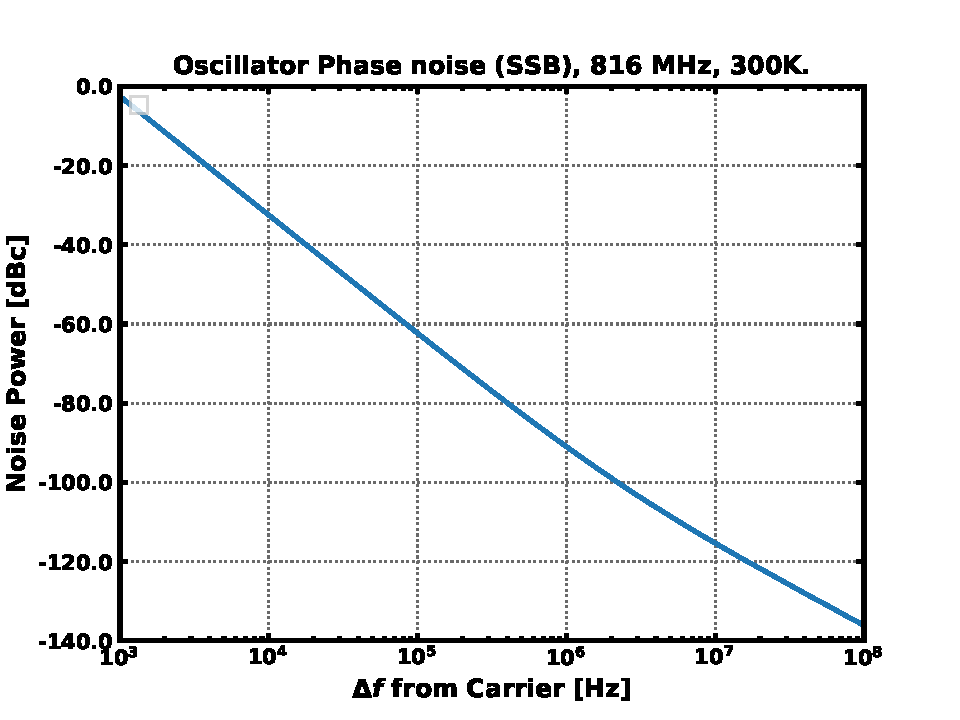
\includegraphics[width=0.65\textwidth, angle=0]{./figs/results/osc_pnoise}
		    \caption{Ring oscillator phase noise (SSB).}
		    \label{fig:ro_pnoise}
		\end{figure}
	\FloatBarrier


	\subsubsection{Tuning}
		\begin{table}[h!]
			\centering
			\def\arraystretch{1.5}		
			\setlength\arrayrulewidth{0.75pt}
			\setlength{\tabcolsep}{1em} % for the horizontal padding
			\begin{tabular}{|l|r|l|r|l|}
				\hline 
				\rule[-1ex]{0pt}{2.5ex} \cellcolor{gray!40}\textbf{Mode} & \cellcolor{gray!40}\textbf{VCO Gain} & \cellcolor{gray!40}\textbf{Units} & \cellcolor{gray!40}\textbf{Normalized gain}& \cellcolor{gray!40}\textbf{Units}\\ 
				\hline 
				\rule[-1ex]{0pt}{2.5ex} \textbf{Supply tuning}  & 2.588 & MHz/mV & 317.2 &\%/V\\
				\hline 
				\rule[-1ex]{0pt}{2.5ex} \textbf{Medium tuning}  & 30.92 & kHz/mV  & 3.789 &\%/V\\
				\hline 
				\rule[-1ex]{0pt}{2.5ex} \textbf{Fine tuning}  & 5.378 & kHz/mV & 0.659 & \%/V\\
				\hline 
				\rule[-1ex]{0pt}{2.5ex} \textbf{Capacitor tuning} & 9782 & kHz/cap & 1.19 & \%/cap\\
				\hline 
			\end{tabular} 
			% \caption{Assigned specifications for branch line hybrid design.}
			% \label{asgn_specs}
			\caption{PLL parameters determined from filter design and optimization process for fast lock speed with TDC feedback.}
			\label{filter_params_fast_lock}
		\end{table} 

	\begin{figure}[htb!]
	    \centering
	    \begin{subfigure}{0.5\textwidth}
	        \centering
	        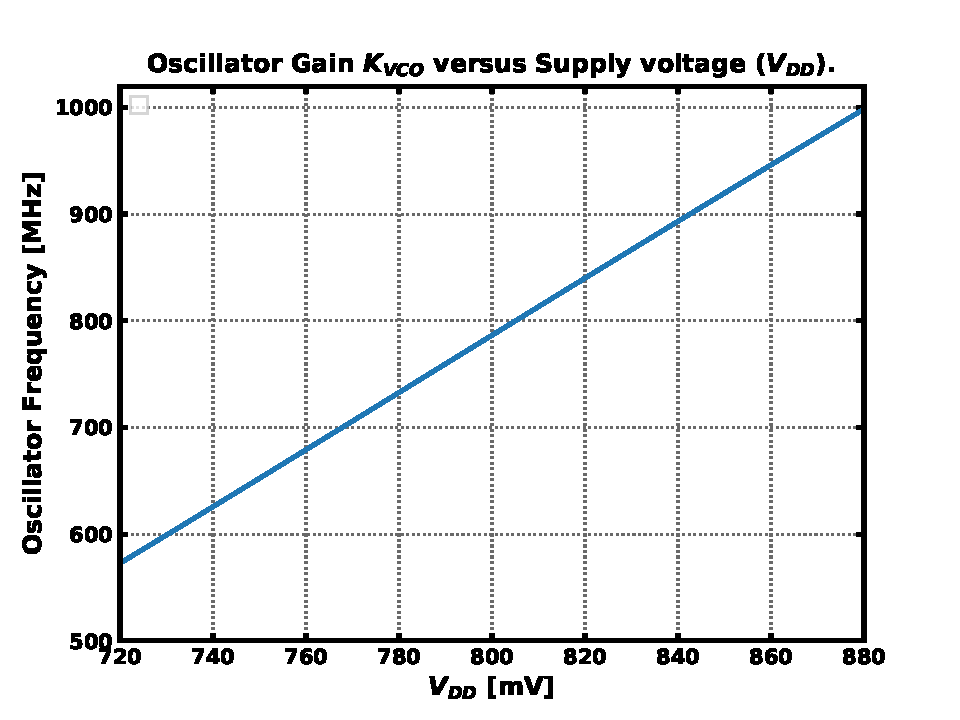
\includegraphics[width=1\textwidth, angle=0]{./figs/results/osc_f_vs_vdd}
	        \caption{ }
	        \label{fig:osc_f_vs_vdd}
	    \end{subfigure}%
	    \begin{subfigure}{0.5\textwidth}
	        \centering
	        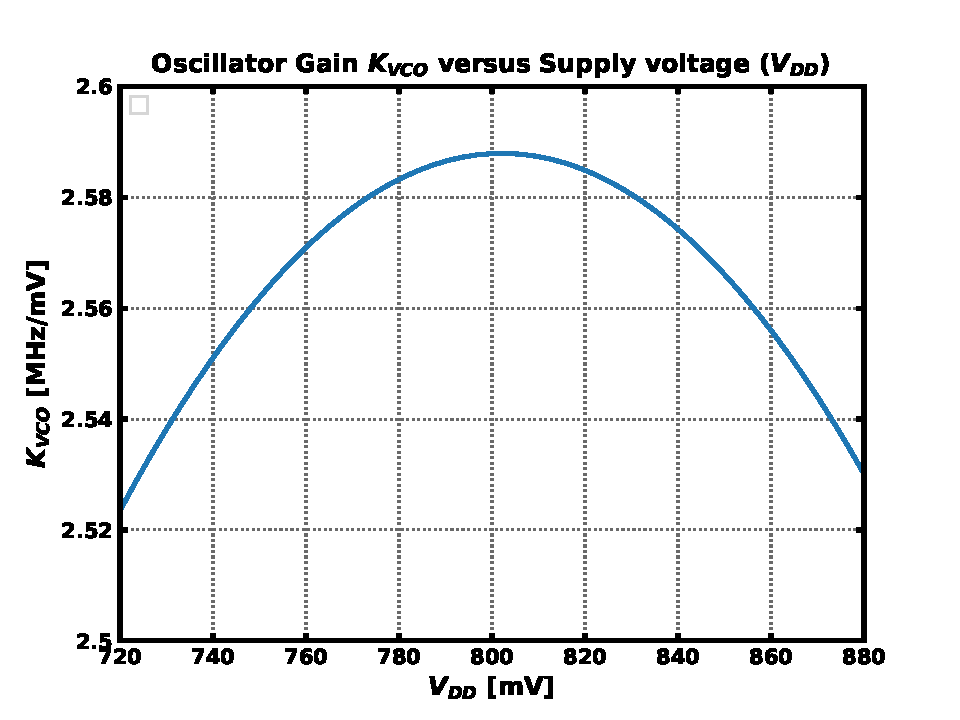
\includegraphics[width=1\textwidth, angle=0]{./figs/results/osc_f_gain_vs_vdd}
	        \caption{ }
	        \label{fig:osc_f_gain_vs_vdd}
	    \end{subfigure}
	    % \caption{x.}
	    \label{fig:osc_f_vdd}
	    \caption{Supply voltage versus ($\pm$ 10\% from 0.8V) \textbf{(a)} Oscillation Frequency, \textbf{(b)} VCO gain.}
	\end{figure} 

	\begin{figure}[htb!]
	    \centering
	    \begin{subfigure}{0.5\textwidth}
	        \centering
	        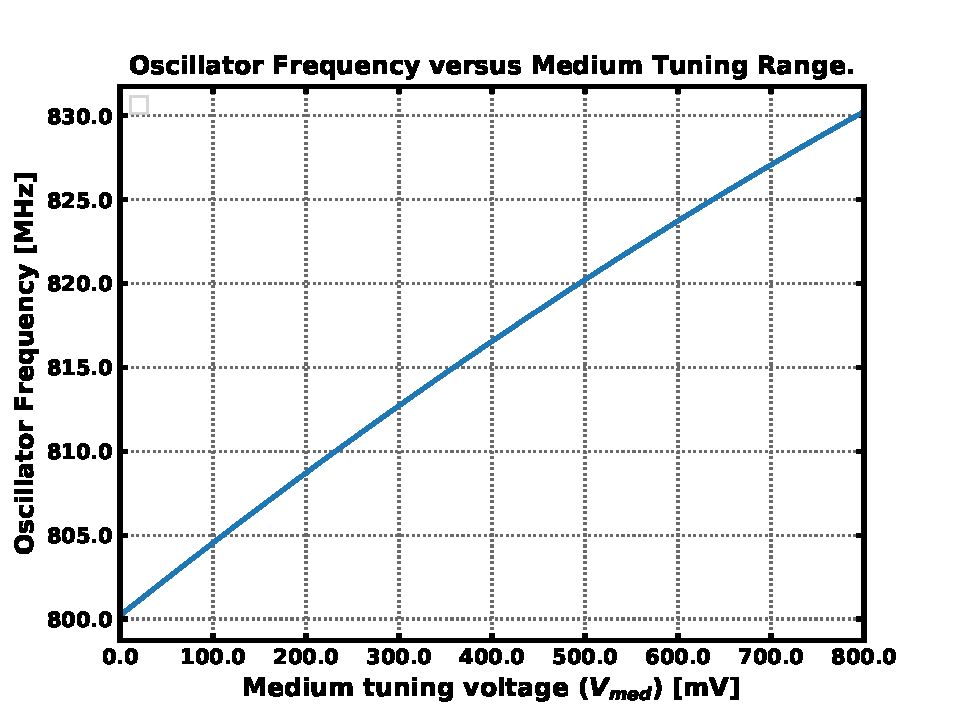
\includegraphics[width=1\textwidth, angle=0]{./figs/results/osc_f_vs_med}
	        \caption{ }
	        \label{fig:osc_f_vs_med}
	    \end{subfigure}%
	    \begin{subfigure}{0.5\textwidth}
	        \centering
	        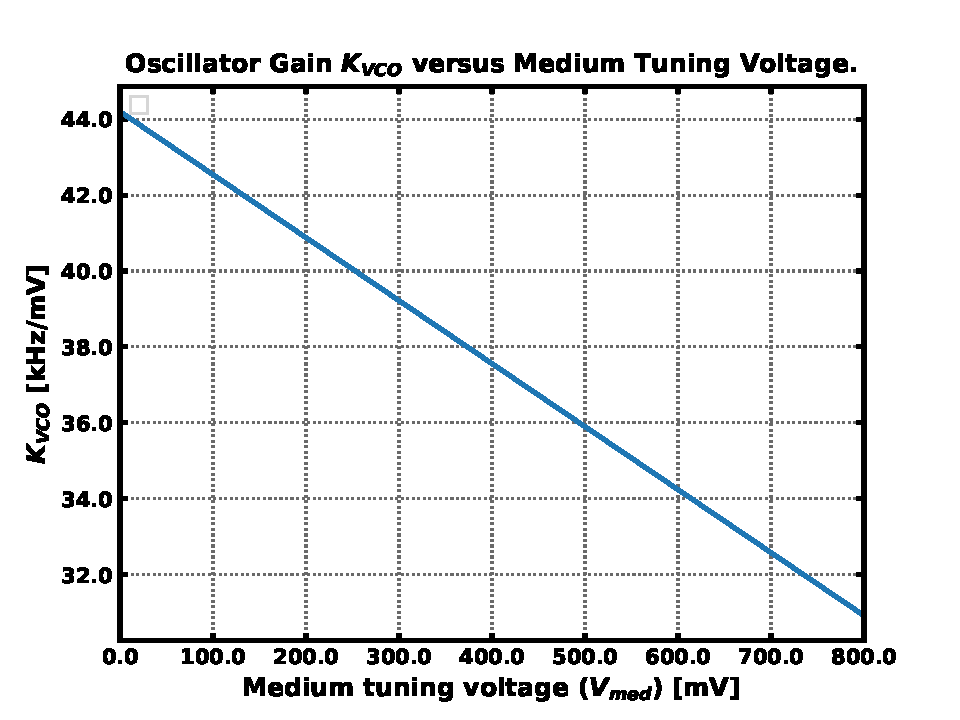
\includegraphics[width=1\textwidth, angle=0]{./figs/results/osc_f_gain_vs_med}
	        \caption{ }
	        \label{fig:osc_f_gain_vs_med}
	    \end{subfigure}
	    % \caption{x.}
	    \label{fig:osc_f_med_tune}
	    \caption{Medium tuning range versus \textbf{(a)} Oscillation Frequency, \textbf{(b)} VCO gain.}
	\end{figure} 


	\begin{figure}[htb!]
	    \centering
	    \begin{subfigure}{0.5\textwidth}
	        \centering
	        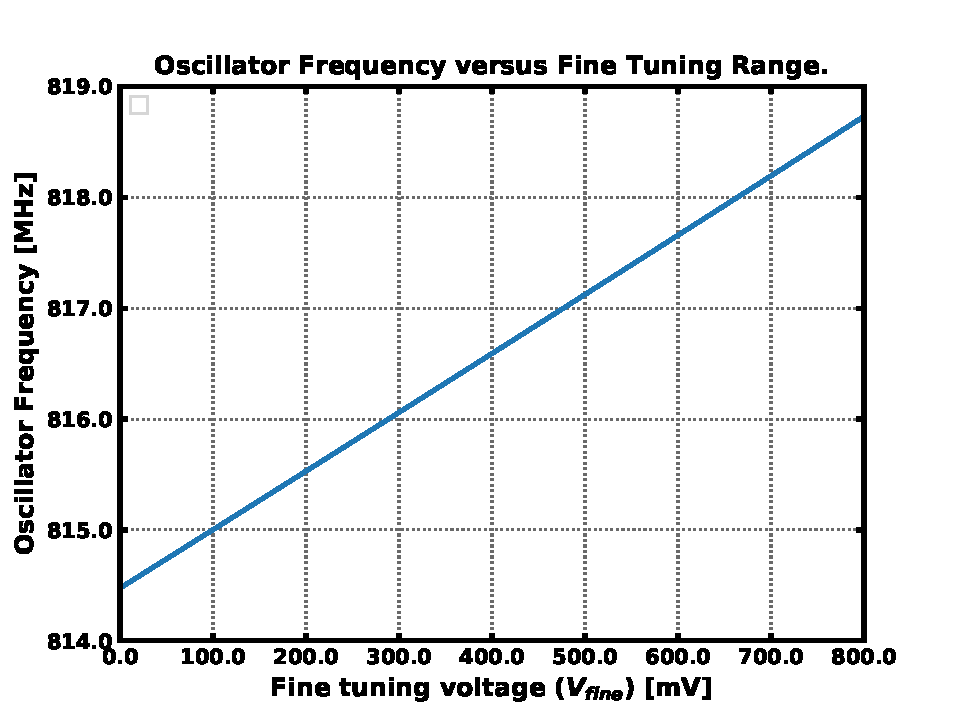
\includegraphics[width=1\textwidth, angle=0]{./figs/results/osc_f_vs_fine}
	        \caption{ }
	        \label{fig:osc_f_vs_fine}
	    \end{subfigure}%
	    \begin{subfigure}{0.5\textwidth}
	        \centering
	        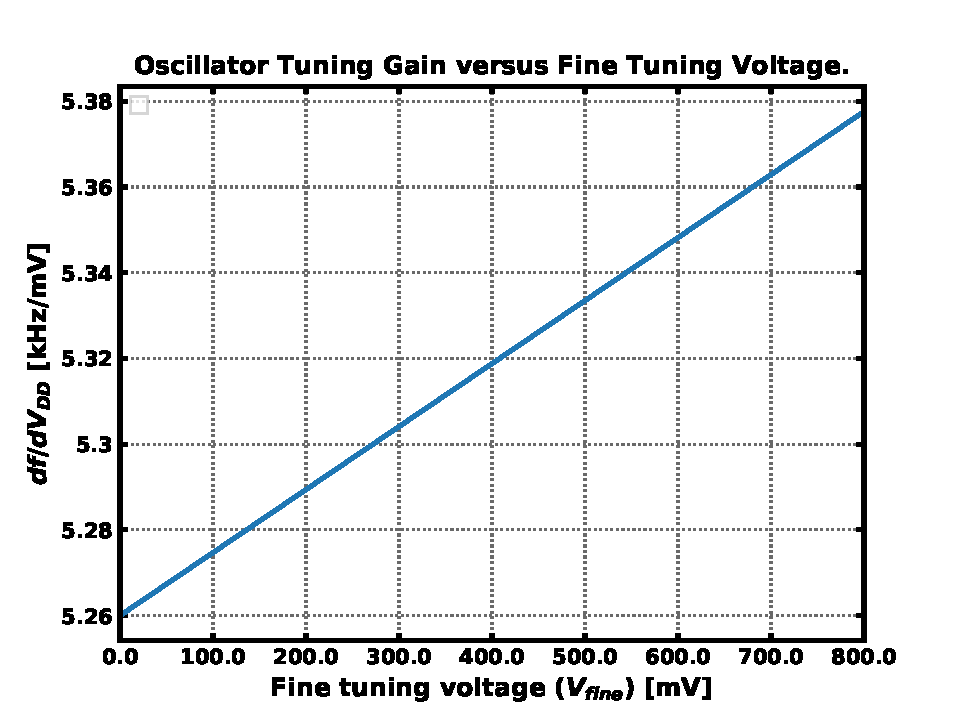
\includegraphics[width=1\textwidth, angle=0]{./figs/results/osc_f_gain_vs_fine}
	        \caption{ }
	        \label{fig:osc_f_gain_vs_fine}
	    \end{subfigure}
	    % \caption{x.}
	    \label{fig:osc_f_fine_tune}
	    \caption{Fine tuning range versus \textbf{(a)} Oscillation Frequency, \textbf{(b)} VCO gain.}
	\end{figure} 

	\FloatBarrier
	\subsubsection{Waveforms}
			\begin{figure}[htb!]
			    \centering
			    \begin{subfigure}{0.5\textwidth}
			        \centering
			        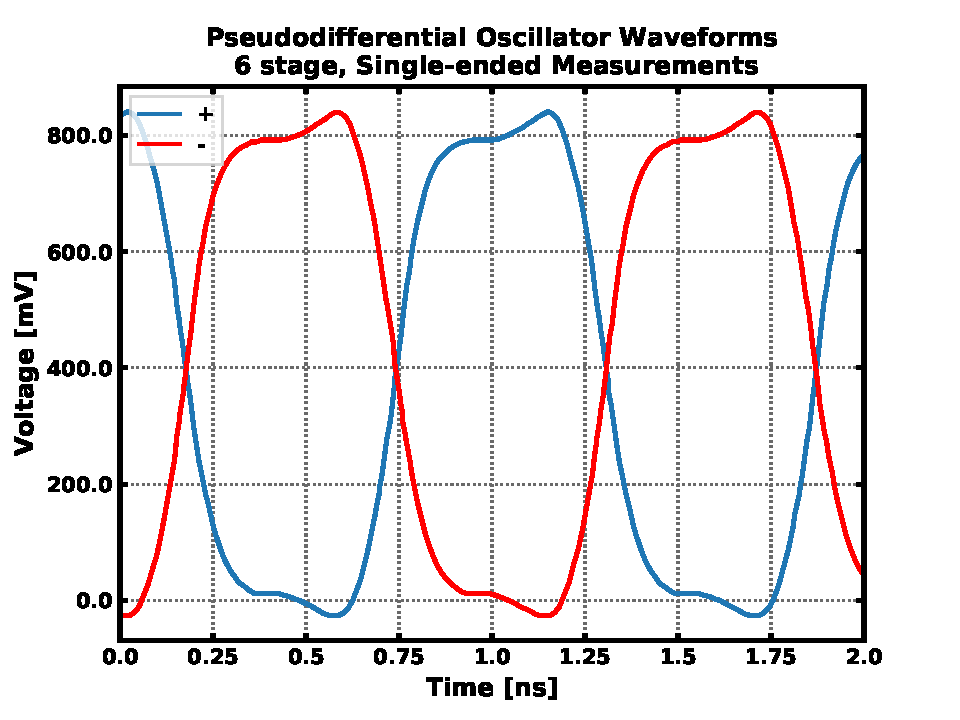
\includegraphics[width=1\textwidth, angle=0]{./figs/results/osc_se_waves}
			        \caption{ }
			        \label{fig:osc_se_waves}
			    \end{subfigure}%
			    \begin{subfigure}{0.5\textwidth}
			        \centering
			        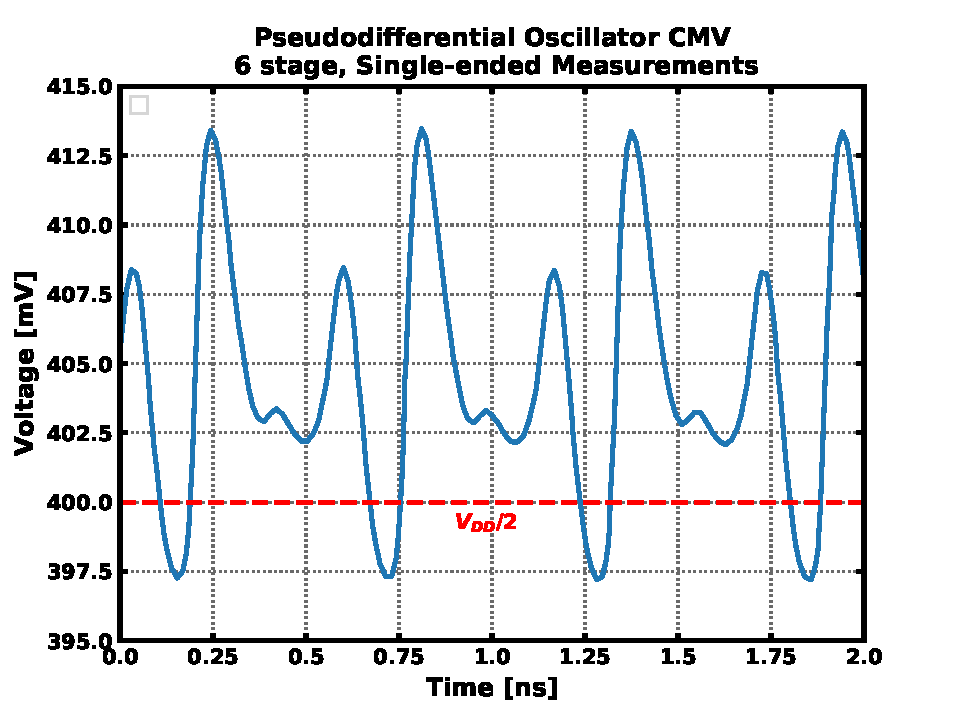
\includegraphics[width=1\textwidth, angle=0]{./figs/results/osc_cmv}
			        \caption{ }
			        \label{fig:osc_cmv}
			    \end{subfigure}
			    % \caption{x.}
			    \label{fig:osc_waves}
			    \caption{\textbf{(a)} Oscillator single-ended waveforms, \textbf{(b)} Oscillator common mode voltage waveform.}
			\end{figure} 
	\FloatBarrier

\subsection{10b CDAC}
	Unit cap = 2.185 fF, total= 2.24pF
	\hl{INL/DNL, unit cap, area}

	\begin{figure}[htb!]
	    \centering
	    \begin{subfigure}{0.5\textwidth}
	        \centering
	        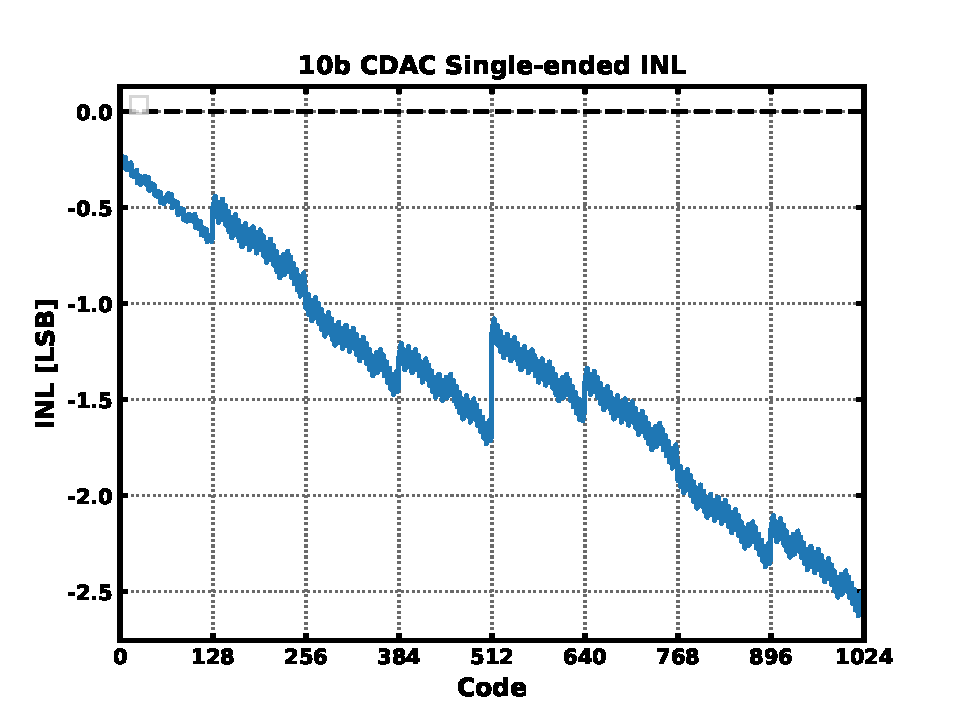
\includegraphics[width=1\textwidth, angle=0]{./figs/results/10b_cdac_se_inl}
	        \caption{ }
	        \label{fig:10b_cdac_se_inl}
	    \end{subfigure}%
	    \begin{subfigure}{0.5\textwidth}
	        \centering
	        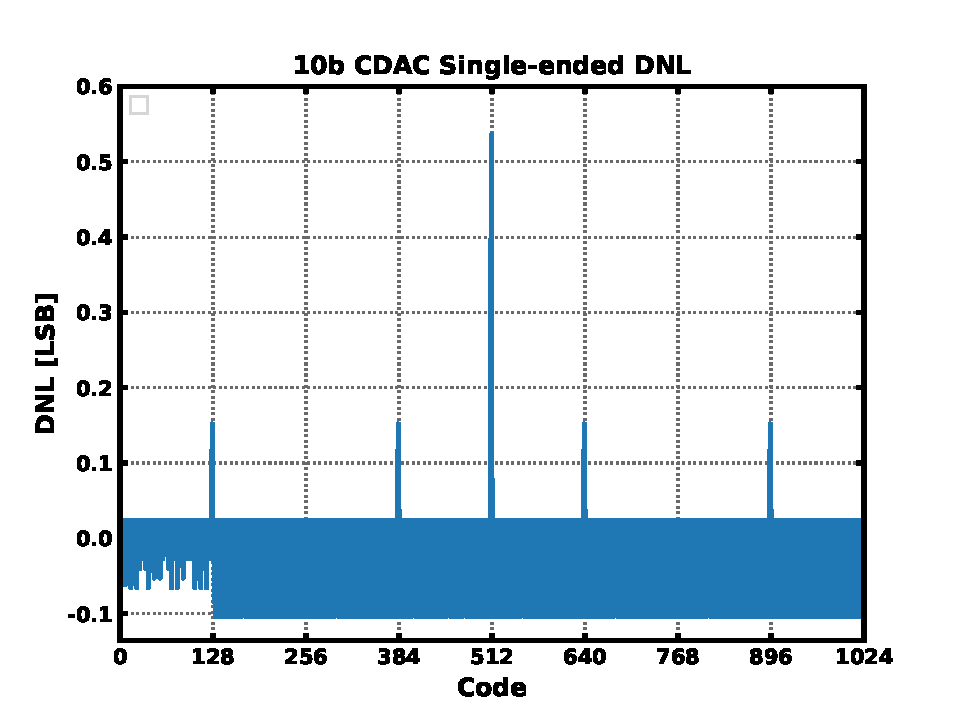
\includegraphics[width=1\textwidth, angle=0]{./figs/results/10b_cdac_se_dnl}
	        \caption{ }
	        \label{fig:10b_cdac_se_dnl}
	    \end{subfigure}
	    % \caption{x.}
	    \label{fig:10b_cdac_se_nonlinearity}
	    \caption{10b CDAC single-ended \textbf{(a)} Integral Nonlinearity, \textbf{(b)} Differential Nonlinearity.}
	\end{figure} 



	\begin{figure}[htb!]
	    \centering
	    \begin{subfigure}{0.5\textwidth}
	        \centering
	        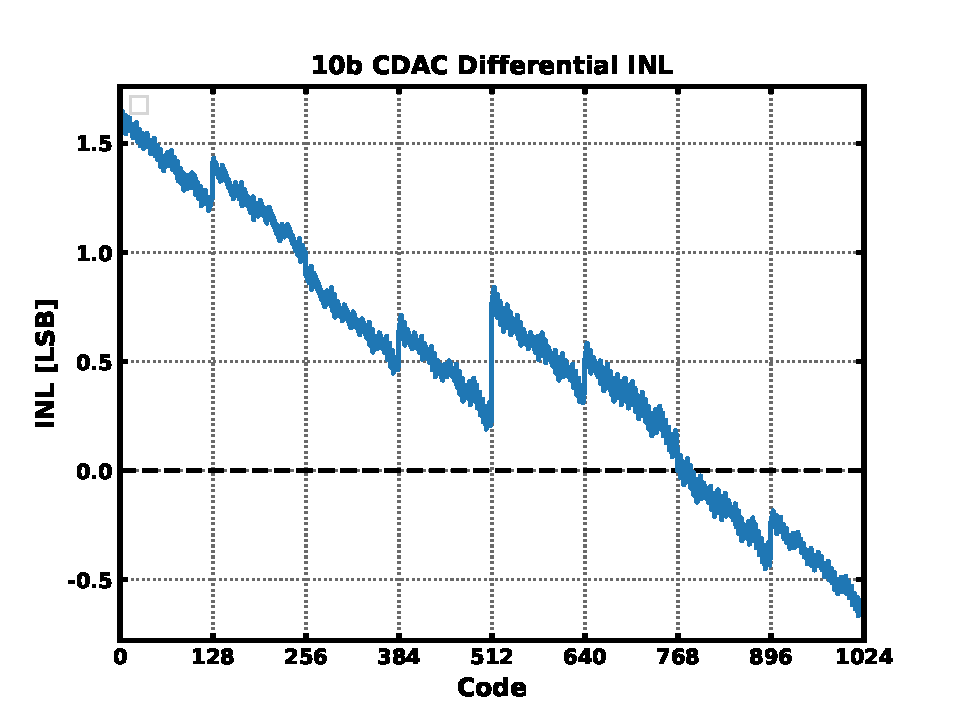
\includegraphics[width=1\textwidth, angle=0]{./figs/results/10b_cdac_diff_inl}
	        \caption{ }
	        \label{fig:10b_cdac_diff_inl}
	    \end{subfigure}%
	    \begin{subfigure}{0.5\textwidth}
	        \centering
	        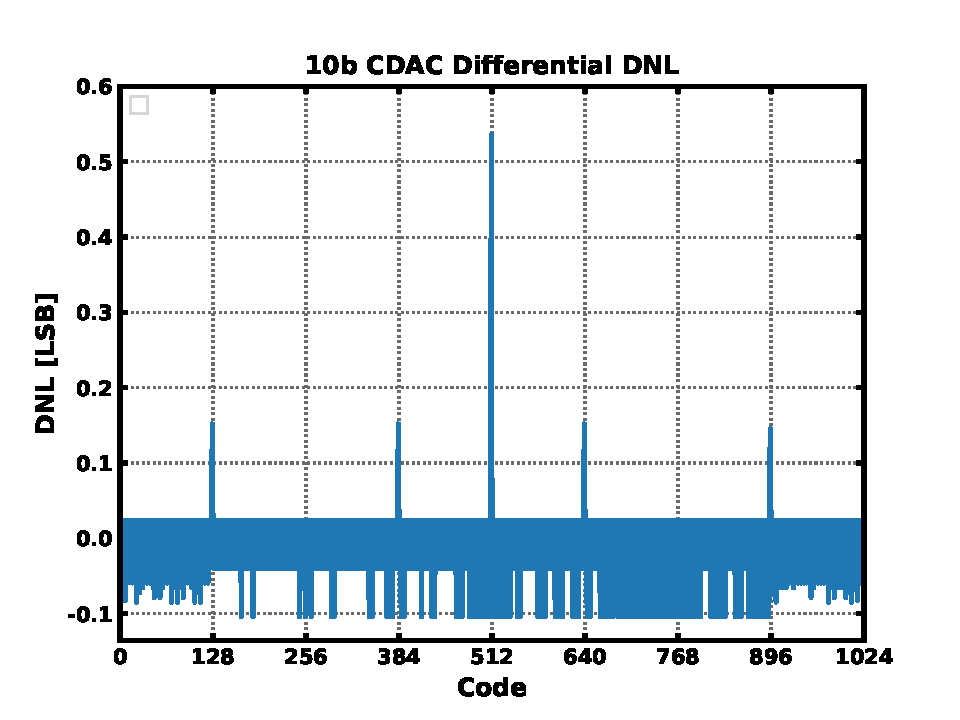
\includegraphics[width=1\textwidth, angle=0]{./figs/results/10b_cdac_diff_dnl}
	        \caption{ }
	        \label{fig:10b_cdac_diff_dnl}
	    \end{subfigure}
	    % \caption{x.}
	    \label{fig:10b_cdac_diff_nonlinearity}
	    \caption{10b CDAC differential \textbf{(a)} Integral Nonlinearity, \textbf{(b)} Differential Nonlinearity.}
	\end{figure} 

\subsection{3b CDAC}
Unit cap = 254fF, total = 2.032pF (tried to get approximately same as 10b CDAC)
\hl{INL/DNL, unit cap, area}

	\begin{figure}[htb!]
	    \centering
	    \begin{subfigure}{0.5\textwidth}
	        \centering
	        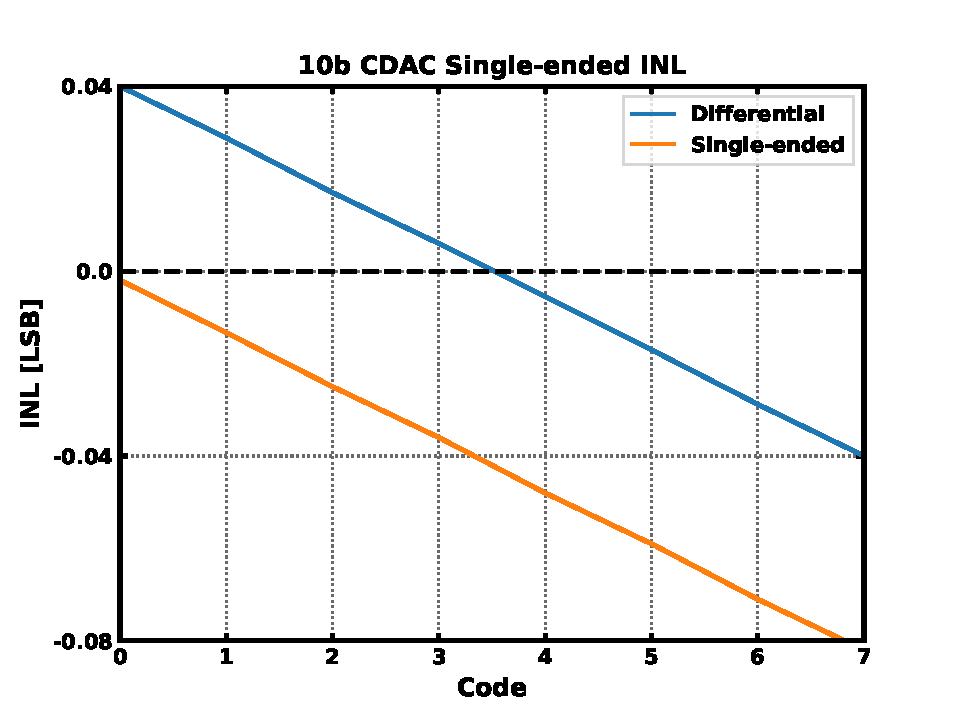
\includegraphics[width=1\textwidth, angle=0]{./figs/results/cdac_3b_inl}
	        \caption{ }
	        \label{fig:cdac_3b_inl}
	    \end{subfigure}%
	    \begin{subfigure}{0.5\textwidth}
	        \centering
	        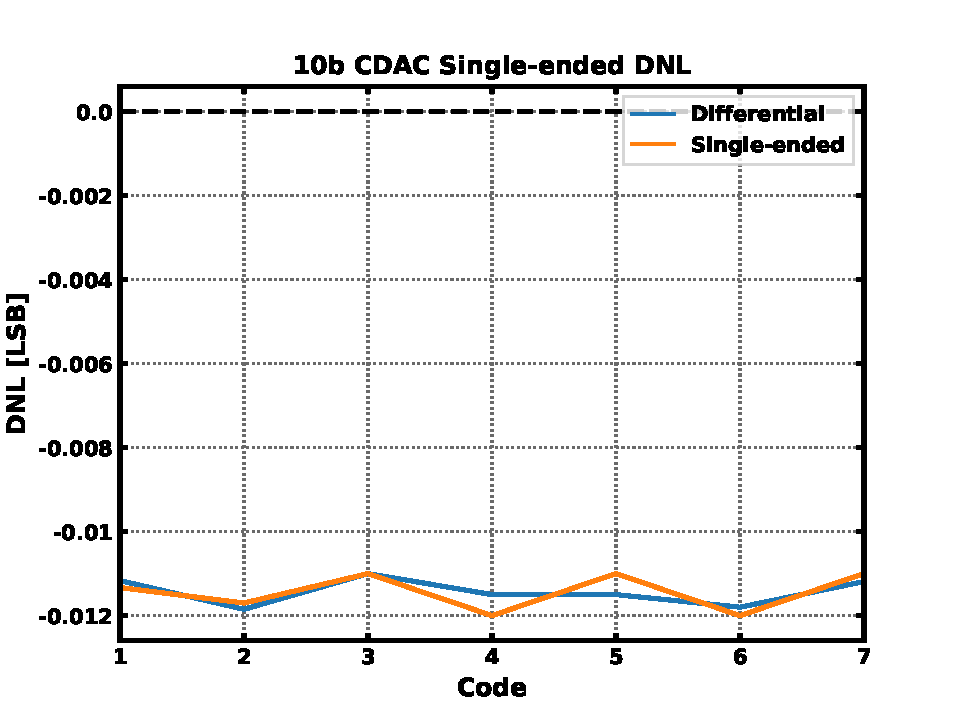
\includegraphics[width=1\textwidth, angle=0]{./figs/results/cdac_3b_dnl}
	        \caption{ }
	        \label{fig:cdac_3b_dnl}
	    \end{subfigure}
	    % \caption{x.}
	    \label{fig:3b_cdac_nonlinearity}
	    \caption{3b CDAC differential \textbf{(a)} Integral Nonlinearity, \textbf{(b)} Differential Nonlinearity.}
	\end{figure} 



\subsection{Bang-bang phase detector}
Noise up to 20 GHz, 100 transitions averaged for 101 delay values, 0.8V, 1.342ps rms jitter added.

	\begin{figure}[htb!]
	    \centering
	    \begin{subfigure}{0.5\textwidth}
	        \centering
	        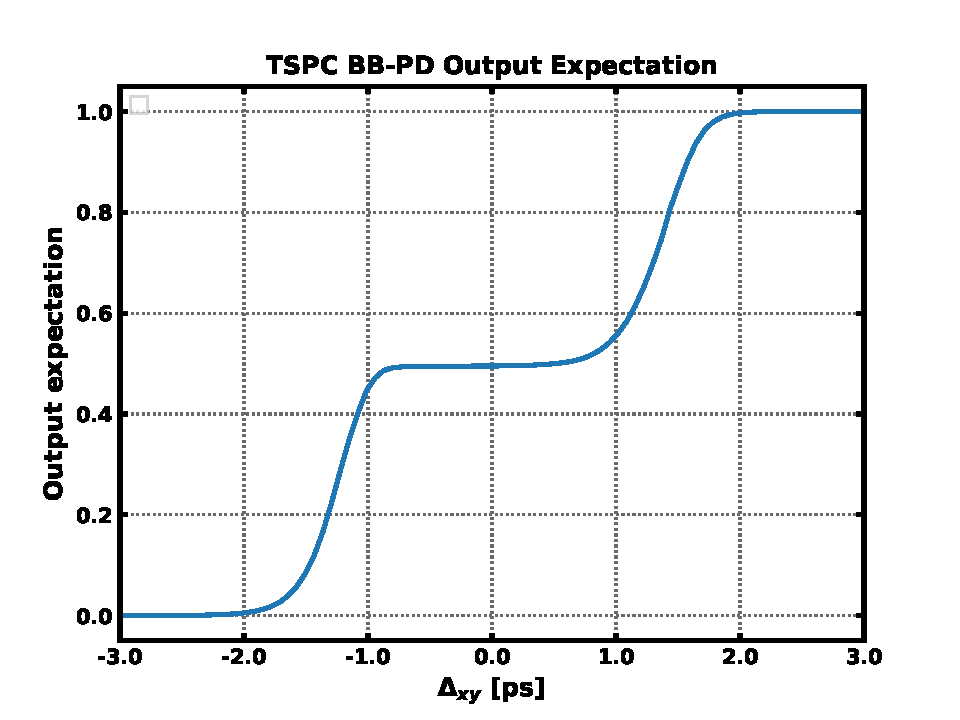
\includegraphics[width=1\textwidth, angle=0]{./figs/results/cdf}
	        \caption{ }
	        \label{fig:bbpd_cdf}
	    \end{subfigure}%
	    \begin{subfigure}{0.5\textwidth}
	        \centering
	        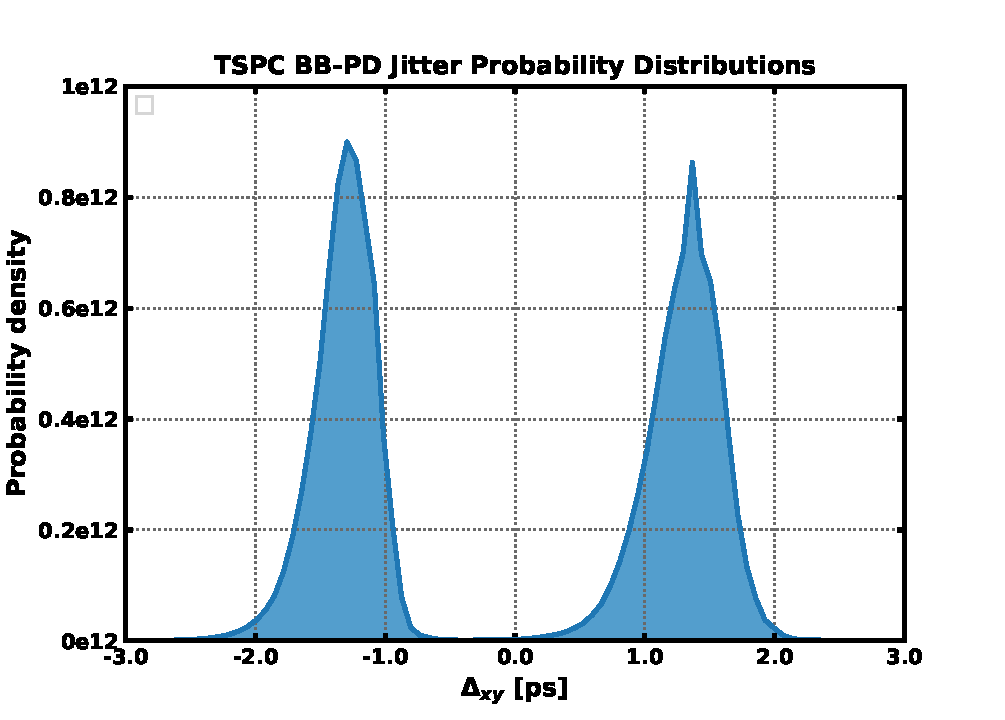
\includegraphics[width=1\textwidth, angle=0]{./figs/results/pdf}
	        \caption{ }
	        \label{fig:bbpd_pdf}
	    \end{subfigure}
	    % \caption{x.}
	    \label{fig:bbpd_jitter_dist}
	    \caption{BBPD extracted jitter \textbf{(a)} Cumulative Distribution Function, \textbf{(b)} Probability Distribution Function.}
	\end{figure} 

\subsection{Logic}
Power consumption

\subsection{Synchronous counter}
Power consumption